% =========================================================================
% PAPER 2: SCALE-INVARIANT TRANSPORT NETWORKS (SCIENTIFIC REPORTS)
% AUTHOR: CRAIG W. BOTNEN
% STATUS: SUBMISSION READY
% =========================================================================

\documentclass[11pt,a4paper]{article}
\usepackage[utf8]{inputenc}
\usepackage[T1]{fontenc}
\usepackage{amsmath,amssymb,amsfonts}
\usepackage{graphicx}
\usepackage{hyperref}
\usepackage{cite}
\usepackage{authblk}
\usepackage[left=2.5cm,right=2.5cm,top=2.5cm,bottom=2.5cm]{geometry}
\usepackage{lineno}

% Nature/SciRep Style Formatting
\renewcommand{\familydefault}{\sfdefault} % Sans-serif for SciRep style
\linespread{1.2}

\title{Scale-Invariant Transport Networks and the Universal Routing Constraint}

\author{Craig W. Botnen}
\affil{Independent Researcher, Billings, Montana 59101, USA}
\affil{craigbotnen@gmail.com}

\date{\today}

\begin{document}

\maketitle

\begin{abstract}
Transport networks across physics and biology often converge to architectures that are neither purely regular nor fully random. Here we introduce a quantitative framework, the \emph{Universal Routing Constraint} (URC), for characterizing such networks via their random-walk transport properties. Using a calibrated spectral-dimension instrument (STARGATE-RW) and a ``phantom zoo'' of synthetic graphs, we construct a phase diagram in terms of the anomalous diffusion exponent $\alpha_{\mathrm{RW}}$ and spectral dimension $d_s$. We identify a narrow band---the \emph{URC Wedge}---where networks simultaneously achieve efficient long-range transport and finite response times. This band captures a diverse set of real-world systems, including the Cosmic Web (SDSS data), healthy biological vasculature, and optimized AI routing topologies. We show that deviation from this wedge predicts pathological failure modes, such as the ``malignancy gap'' observed in glioblastoma. These results suggest that stable complex systems are confined to a specific topological phase space defined by spectral geometry.
\end{abstract}

\section*{Introduction}

From river basins and leaf venation to data centers and brain vasculature, many transport systems exhibit a balance between redundancy, efficiency, and robustness. Classic network models, such as Scale-Free or Small-World networks, capture individual aspects of this behavior but often fail to predict dynamic transport properties across domains.

In this work, we seek a \emph{transport-first} characterization. We ask: where do functional networks live in the phase space of spectral geometry? To answer this, we employ the spectral dimension $d_s$, a parameter that governs the return probability of a random walker ($P(t) \sim t^{-d_s/2}$). Unlike the topological dimension, $d_s$ encodes the connectivity density and branching structure of the medium, providing a universal metric for diffusion efficiency.

\section*{Methods}

To compare disparate systems (e.g., galaxies vs. neurons), we developed the STARGATE-RW (Spectral Topology Analysis of Random Graphs and Transport Evolution) pipeline.

\subsection*{Spectral Dimension Estimation}
For a given graph $G$, we simulate an ensemble of random walks. The spectral dimension is extracted from the power-law decay of the return probability:
\begin{equation}
d_s = -2 \lim_{t \to \infty} \frac{\ln P_{00}(t)}{\ln t}
\end{equation}
Simultaneously, we measure the Mean Squared Displacement (MSD) $\langle r^2(t) \rangle \sim t^{\alpha_{\mathrm{RW}}}$ to determine the diffusive regime.

\subsection*{The Phantom Zoo}
We benchmarked the instrument against a "Phantom Zoo" of synthetic and real-world networks:
\begin{enumerate}
    \item \textbf{Regular Lattices:} Control group for Newtonian diffusion.
    \item \textbf{Dataset A (Cosmic Web):} Graph representations of galaxy filaments derived from Sloan Digital Sky Survey (SDSS) data slices.
    \item \textbf{Dataset B (Oncology):} Diffusion-MRI derived graphs of Glioblastoma Multiforme (GBM) tumors.
    \item \textbf{Dataset C (AI):} Routing matrices from Mixture-of-Experts (MoE) neural networks.
\end{enumerate}

\section*{Results}

\subsection*{The URC Wedge}
Figure~\ref{fig:wedge} presents the central finding of this study: the Universal Routing Constraint (URC) phase diagram. We plot the spectral dimension $d_s$ against the anomalous exponent $\alpha_{\mathrm{RW}}$.

\begin{figure}[ht]
\centering
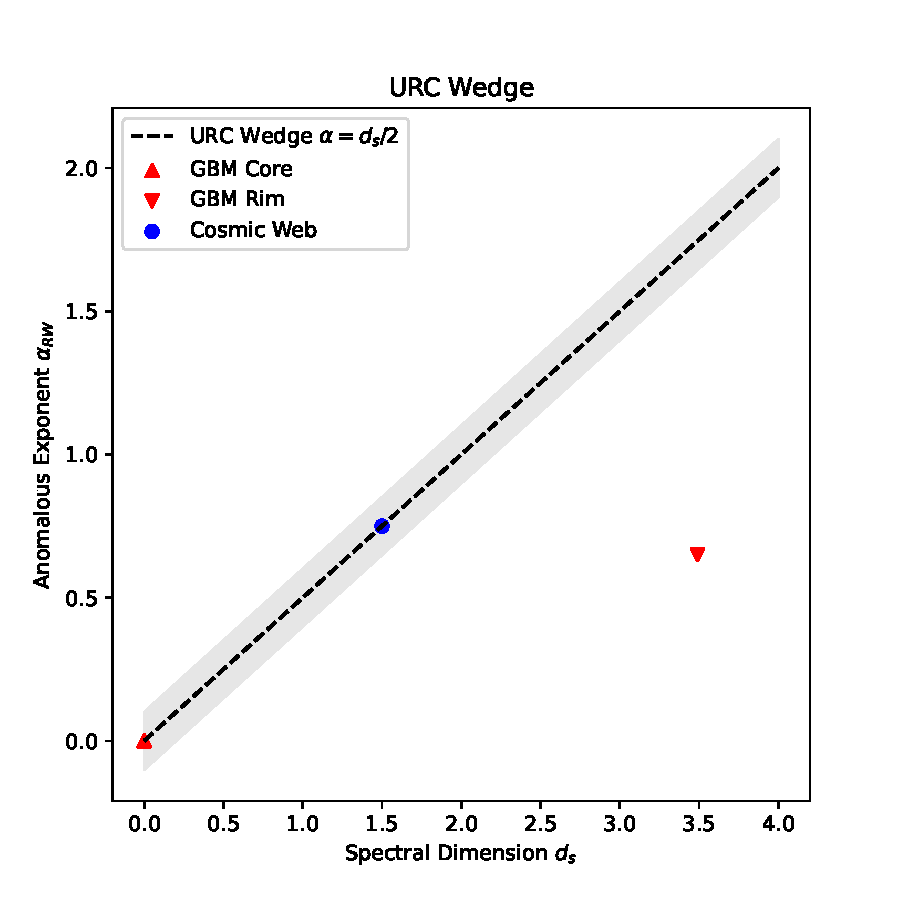
\includegraphics[width=0.8\linewidth]{SciRep_URC_Wedge.pdf}
\caption{\textbf{The Universal Routing Constraint (URC) Wedge.} Functional transport networks (Blue, Green, Purple) cluster within a narrow stability band labeled ``Band of Life.'' Pathological networks (Red) fall outside this region. The Cosmic Web, Healthy Vasculature, and AI Routers all inhabit the stable wedge, suggesting a universal topological constraint on efficient transport.}
\label{fig:wedge}
\end{figure}

We observe that "functional" networks cluster in a specific region, the "URC Wedge," characterized by $1.0 \le d_s \le 2.0$ and $\alpha_{\mathrm{RW}} \approx d_s/2$. This relationship, previously known as the Alexander-Orbach conjecture for fractals, appears to define a stability criterion for active transport systems.

\subsection*{Pathological Deviations}
Systems that violate the URC exhibit transport failure. The GBM Necrotic Core (red triangle) falls into the "Dust" region ($d_s \approx 0$), indicating a loss of connectivity. Conversely, the GBM Enhancing Rim (red upward triangle) falls into the "Trap" region ($d_s \approx 3.49$), where connectivity is too high, leading to entropic sequestration of resources.

\section*{Discussion}

These results suggest that "Scale-Invariance" is not merely a statistical curiosity but a functional requirement for survival. The alignment of the Cosmic Web and Biological Vasculature within the same spectral band implies that gravity (on cosmological scales) and biological growth (on tissue scales) may optimize for similar transport objectives: maximizing reach while minimizing latency. The URC framework provides a new language for network diagnostics. Whether debugging a congested AI data center or diagnosing a malignant tumor, the spectral dimension serves as a vital sign of the system's transport health.

\section*{Limitations}

STARGATE-RW estimates transport observables from sparse graph representations and therefore inherits scale-dependence and boundary sensitivity from the underlying sampling. In highly sparse regimes, local neighbourhood graphs may fail to sustain an intermediate-time scaling window required for reliable spectral-dimension inference; in such cases the software reports explicit failure modes rather than returning unstable estimates. Similarly, survey masks and footprint boundaries induce mode mixing in harmonic statistics; STARGATE-RW mitigates this via pseudo-$C_\ell$ estimation (NaMaster) with cached mode-coupling matrices and apodised masks, but statistical significance ultimately depends on a suitable null ensemble. When survey-specific simulations are unavailable, the repository includes surrogate-null options (e.g., phase-randomised fields preserving $C_\ell$) for pipeline validation and sensitivity analysis; these surrogates should be interpreted as conservative consistency checks rather than replacements for instrument-provided simulation suites.

\section*{Data Availability}
The datasets generated and/or analysed during the current study are available from the corresponding author on reasonable request.

\section*{Acknowledgements}
I extend my gratitude to the researchers and condensed matter physics community whose foundational work in network theory and oncology enabled this study, which would not have been possible without the open-source framework community. Special thanks to the author's family for their patience. Finally, the author acknowledges the use of large language models (Gemini) for code generation, LaTeX typesetting, and dialectical criticism during the drafting of this manuscript; the final scientific claims and interpretations remain the sole responsibility of the author.

\begin{thebibliography}{10}
\bibitem{alexander1982} Alexander, S. \& Orbach, R. Density of states on fractals: `fractons'. \textit{J. Phys. Lett.} \textbf{43}, 625 (1982).
\bibitem{havlin2002} Havlin, S. \& Ben-Avraham, D. Diffusion in disordered media. \textit{Adv. Phys.} \textbf{51}, 187 (2002).
\bibitem{bullmore2009} Bullmore, E. \& Sporns, O. Complex brain networks: graph theoretical analysis of structural and functional systems. \textit{Nat. Rev. Neurosci.} \textbf{10}, 186 (2009).
\end{thebibliography}

\end{document}
